\chapter{Sherical vs non-spherical wrist robots} \label{sec:SphericalVsNonspherical}

Robots with a spherical axis configuration usually have three rotating wrist axes that intersect at one point while non-spherical configurations have a shifted wrist axis, see figure \ref{fig:SphericalVsNonspherical}.
This leads to different solutions in the inverse kinematics. Spherical wrist robots have up to 8 solutions for the same endeffector position while non-spherical have 9.
Spherical wrist robots have a simpler inverse kinematic solution, while suffering from more singularities. \cite{SphericalNonspherical}



\begin{figure}[H]
	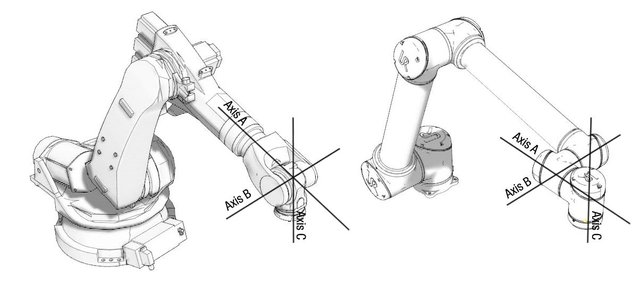
\includegraphics[
	width=1\linewidth,
	center,
	keepaspectratio,
	]{SphericalVsNonspherical}
	\caption{Spherical vs non-spherical wrist robots \cite{SphericalNonspherical}}
	\label{fig:SphericalVsNonspherical}
\end{figure}